\documentclass[12pt]{article}

% PACKAGES
\usepackage[ngerman]{babel}
\usepackage{lmodern} % Schriftart
\usepackage{bookmark} % Für PDF Lesezeichen
\usepackage{caption} % Für \caption*{}
\usepackage{siunitx} % SI-Einheiten
\usepackage{mathtools} % Verbessertes "amsmath" (https://de.overleaf.com/learn/latex/Articles%2FMathtools_-_for_beautiful_math)
\usepackage{xcolor}   % Farbiger Text (https://www.overleaf.com/learn/latex/Using_colours_in_LaTeX)
\usepackage{geometry} % Zur Einstellung des Layouts
\usepackage{titlesec} % Einteilung des Inhalts (https://de.overleaf.com/learn/latex/Sections_and_chapters)
\usepackage{fancyhdr} % Für Kopf-/ und Fußzeilen (https://www.overleaf.com/learn/latex/Headers_and_footers)
\usepackage{parskip} % Änderung von Absätzen und Absatzeinzügen
\usepackage{biblatex} % Verweise und Referenzen
\usepackage{float} % Benötogt für Figuren und Tabellen
\usepackage{graphicx} % Platzhalter Bilder
\usepackage{booktabs} % Tabellen
\usepackage{csquotes} % Recommended package for biblatex
\usepackage{hyphenat}
% SETUP 
\setlength{\headheight}{14.5pt} % Set headheight to at least 14.5pt
\addtolength{\topmargin}{-2.5pt} % Make topmargin smaller to compensate
\sisetup{
  per-mode=fraction,
  fraction-function=\tfrac,
  separate-uncertainty=true
}
\addbibresource{Ressourcen/V44.bib}
\geometry{ %A4
  a4paper,
  total = {170mm,240mm},
  left = 20mm,
  top = 30mm
}
\pagestyle{fancy}
\captionsetup[figure]{
    justification=centering, % Centered captions
    labelsep=colon, % Separate label and caption with a period
    singlelinecheck=false, % Always center even if the caption is short
    labelfont=bf % Bold captions
}
% COMMANDS
\newcommand{\uproman}[1]{\uppercase\expandafter{\romannumeral#1}} % Römische Zahlen


% DOC
\begin{document}

% HEADER
\begin{titlepage}
  \centering
  \vspace*{1cm}
  
\includegraphics[width=0.5\textwidth]{Ressourcen/tud_logo_schwarz(RGB)}\\
  \vspace*{0.25cm}
  \large\textmd{Fakultät Physik} \\
  \vspace*{6cm}
  \huge \bfseries FP-2024 - Versuch V44\\
  \vspace*{0.25cm}
  \large Röntgenreflektometrie\\
  \vspace*{0.25cm}
  \large\textmd{\href{mailto:martin.boussard@tu-dortmund.de}{Martin Boussard}} \\
  \large\textmd{\href{mailto:jan.oppoli@tu-dortmund.de}{Jan Oppoli}} \\
  \vfill
  \small\textmd{Versuch durchgeführt am 22. April 2024}\\
  \small\textmd{Abgabe erstellt am \today}
\end{titlepage}
\tableofcontents 
\newpage

\section{Zielsetzung}\label{sec:zielsetzung}
Ziel dieses Versuchs ist es, verschiedene physikalische bzw. geometrische Eigenschaften wie Elektronendichte, Schichtdicke oder Rauigkeit eines Polysterolfilms auf einem Siliziumwafer mittels der Röntgen-reflektometrie zu bestimmen.
Die Untersuchung/ Kontrolle solcher Schichten im Nanometerbereich ist insbesondere innerhalb der Halbleiterelektronik von Bedeutung und besitzt eine hohe Relevanz für die Industrie.
Durch Analyse des Resultierenden Streubildes unter Verwendung problemangepasster Algorithmen können charakteristische Strukturinformationen der Probe gewonnen werden.
\section{Theorie}\label{sec:theorie}
Als Grundlage für eine effiziente Auswertung der Daten müssen zunächst einige wichtige physikalische Phänomene bzw. Modelle erläutert werden.
\subsection{Röntgenstrahlung}\label{subsec:röntgen}
Aufgrund ihrer relativ zum sichtbaren Licht vergleichsweise kleine Wellenlänge 
\begin{align*}
  \lambda_{\text{Röntgen}} < \SI{10}{\nano\meter} < \SI{400}{\nano\meter} <\lambda_\text{Sichtbar}
\end{align*}
eignet sich Röntgenstrahlung ideal zur Untersuchung von Strukturen der selben Größenordnung.
\subsubsection{Erzeugung von Röntgenstrahlung}
Nachdem mithilfe des Glühelektrischen Effekts aus der Kathode herausgelöste Elektronen innerhalb der Röntgenröhre in Richtung der Anode beschleunigt werden, wird bei dem Auftreffen Röntgenstrahlung erzeugt.
Hierbei ist zwischen Bremsstrahlung und dem charakteristischen Röntgenspektrum zu unterscheiden, wie in \autoref{fig:1} veranschaulicht ist.
\begin{itemize}
  \item \textbf{Bremsstrahlung}:\\Die durch Coulombwechselwirkung zwischen Elektron und Atomrumpf des Targets verkleinerte kinetische Energie des Elektrons wird teilweise in Röntgenstrahlung mit kontinuierlichem Spektrum umgewandelt und emittiert.
  \item \textbf{Charakteristische Röntgenstrahlung}:\\Treffen die beschleunigten Elektronen auf das Target und lösen dort Elektronen aus inneren Schalen des Atoms heraus, werden diese Leerstellen durch nachrückende Elektronen aus höheren Schalen gefüllt und die resultierende Energiedifferenz spiegelt sich in der Emission von Röntgenstrahlung diskreter Frequenzen wieder, da die Übergangsenergien im Atom quantisiert sind.
\end{itemize}
\begin{figure}[H]
  \centering
  \includegraphics[scale=0.5]{Ressourcen/Röntgenspektrum.png}
  \caption{Schematisches Emissionsspektrum einer Kupferanode, wie auch\\in diesem Versuch verwendet.\cite{ROEDresden}}\label{fig:1}
\end{figure}
\subsubsection{Eigenschaften von Röntgenstrahlung}
Die in diesem Versuch relevanteste Frequenz ist die sog. $\text{K}_\alpha$-Linie, welche einem Übergang eines Elektrons von der zweiten(M) in die erste(K) Schale und der Wellenlänge $\lambda_{\text{K}_\alpha}=\SI{0.1514}{\nano\meter}$ entspricht\cite{ekabs}.
Die zugehörige Frequenz $\omega$ liegt weit über jeglichen Resonanzfrequenzen $\omega_1$ der betrachteten Materialien, was für weitere theoretische Betrachtungen von Bedeutung ist.
\subsubsection{Röntgenstrahlung an Grenzflächen}
Das Verhalten von Röntgenstrahlung an Grenzflächen von Medien unterschiedlichem Brechungsindexes wird gemäß des Snelluis'schen Brechungsgesetzes
\begin{align}
  n_1 \sin(\alpha) = n_2 \sin(\alpha_\text{t})\label{eq:snellius}
\end{align}
in \autoref{fig:2} dargestellt, wobei nach dem Reflexionsgesetz Einfallswinkel = Ausfallswinkel gilt.
\begin{figure}[H]
  \centering
  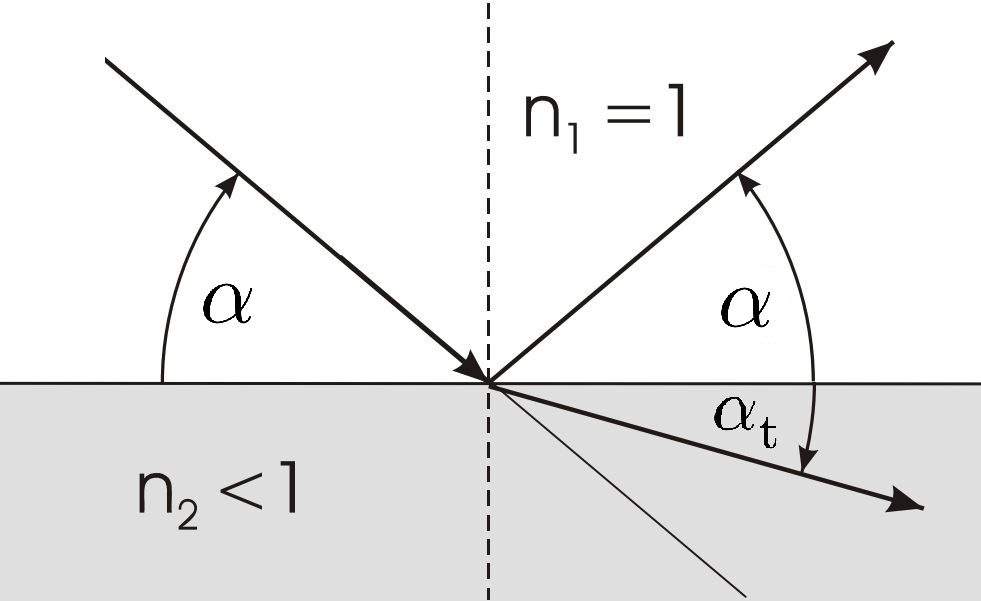
\includegraphics[scale=0.3]{Ressourcen/Snellius.png}
  \caption{Skizze der Winkel des einfallenden, ausfallenden und\\ gebrochenen Strahls and einer Grenzfläche.}\cite{uni_giessen}\label{fig:2}
\end{figure}
Der komplexe Brechungsindex $n$ von verschiedenen Medien rührt von Lorentz-Oszillator-Modell für Fest-körper her, bei welchem sich im hochfrequenten Näherungsfall der Röntgenstrahlung die folgende Formel für nicht-ferromagnetische Materialien  
\begin{align}
  n=\sqrt{\epsilon_\text{r}}=1-\frac{\rho r_0}{2\pi}\lambda^2+i \frac{\gamma}{4\pi}\lambda \coloneqq 1-\delta+i\beta\label{eq:n}
\end{align}
mit Elektronenradius $r_0$, Elektronendichte $N$, Wellenlänge $\lambda$ und linearem Absorptionskoeffizient $\gamma$ zusammengefasst in Kenngrößen der Dispersion $\delta$ und dem Absorption $\beta$, ergibt. 
\\\linebreak Besonderheit der Röntgenstrahlung ist, dass für sie jedes Medium geringfügig optisch dünner als das Vakuum erscheint, womit im Gegensatz zu sichtbarem Licht Totalreflexion im Übergang von Vakuum zu Medium auftreten kann.
Dies tritt gemäß \autoref{eq:snellius}, \ref{eq:n} für Winkel
\begin{align}
  \alpha_\text{Krit} < \sqrt{2 \delta} = \lambda \sqrt{\frac{\rho r_0}{\pi}}
\end{align}
auf.
\section{Auswertung}\label{sec:auswertung}

\section{Diskussion}\label{sec:diskussion}

\section{Literaturverzeichnis}\label{sec:literaturverzeichnis}
\printbibliography[heading = none]
\newpage

\section{Anhang}\label{sec:anhang}

\end{document}
